\documentclass{article} 
\usepackage{xeCJK}
\usepackage{geometry}
\usepackage{mwe}
\usepackage{setspace} 
\usepackage{amsmath}
\usepackage{graphicx}
\usepackage{wrapfig}


%\author{} 
%\title{刘环宇} 
%\date{}
\geometry{left=2.0cm, right=2.0cm, top=1.5cm, bottom=2.5cm}

\begin{document} 


%\maketitle 
\pagestyle{empty}  % no page number for the second and the later pages  
\thispagestyle{empty} % no page number for the first page   


%##############################################################
\begin{minipage}[b]{0.6 \linewidth}
\LARGE \centerline{刘环宇}
\linespread{1.5}\selectfont %需要与前面换行,以保证该句行间距仅对下段文字有效
\large \centerline{(+86) 18868112137 • liuhy@zju.edu.cn}
\large \centerline{https://github.com/liuhyCV}
\large \centerline{}
\large \centerline{}

\end{minipage}
\hfill
\begin{minipage}[b]{0.25 \linewidth}
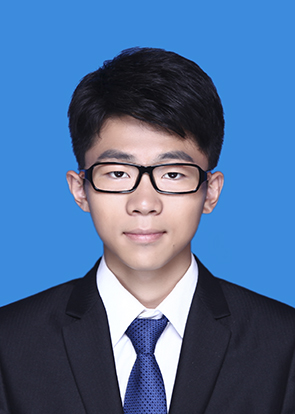
\includegraphics[width=7 \baselineskip]{photo.jpg}
\end{minipage}






%##############################################################
\section*{Education}
\vspace{-1.3\baselineskip}
\noindent\hrulefill

\par \large \textbf{浙江大学},控制科学与工程  \hfill 2012.09—2016.06
\linespread{1.2}\selectfont
\par GPA:4.01/5
\par 浙江大学学生三等学业奖学金(2013-2014)

\par \large \textbf{浙江大学},智能控制与系统  \hfill 2016.09—2019.03
\linespread{1.6}\selectfont %\\表示换行
\par 社会实践单项奖(2016-2017)

\linespread{1.2}\selectfont %需要与前面换行,以保证该句行间距仅对下段文字有效

%##############################################################
%\section*{Publications}
%\vspace{-1.3\baselineskip}
%\noindent\hrulefill




%##############################################################
\section*{Reserarch Experience}
\vspace{-1.3\baselineskip}
\noindent\hrulefill


%###########################
\par \large \textbf{浙江大学}  \hfill 2016.07—2019.03
\linespread{1.6}\selectfont %\\表示换行

\linespread{1.2}\selectfont %需要与前面换行,以保证该句行间距仅对下段文字有效
\par 导师:姜伟
\begin{itemize}
\item \textbf{实例分割}。基于part segmentation和keypoint detection,实现无人驾驶场景中,车辆的实例检测与分割。该研究采取自下而上的方法,基于CNN网络生成part和keypoint,基于二分图和匈牙利算法实现单个实例的组合。
\end{itemize}

\begin{itemize}
\item  \textbf{基于单张图像的场景深度恢复}。从准确度、运行速度、泛化能力、网络结构等角度分析领域研究进展,复现《Depth Map Prediction from a Single Image using Multi-Scale Deep Network》,构建 Multi-Scale CNN 网络,实现 NYU Depth 数据集准确率 0.60(threshold<1.25)
\end{itemize}


%###########################
\par \large \textbf{图森未来算法部}  \hfill 2017.07—2017.10
\linespread{1.6}\selectfont %\\表示换行

\linespread{1.2}\selectfont %需要与前面换行,以保证该句行间距仅对下段文字有效
\par 实习导师:王乃岩、戴恒晨
\begin{itemize}
\item 研究自动驾驶中语义分割的相关算法,复现《ICNet for Real-Time Semantic Segmentation on High-Resolution Images》,在Cityscapes数据集上实现mIoU=0.69 (33ms TitanX GPU);探究了基于不同层次特征融合的相关方法,以及速度和准确率的权衡问题;
\end{itemize}



%###########################
\par \large \textbf{浙江大学}  \hfill 2015.12—2016.05
\linespread{1.6}\selectfont %\\表示换行

\linespread{1.2}\selectfont %需要与前面换行,以保证该句行间距仅对下段文字有效
\par 本科毕设(优秀)  \quad 导师:姜伟
\begin{itemize}
\item \textbf{基于视觉方式的发票自动识别}。针对特定发票图像,设计图像预处理流程,基于 Gabor 特征、分类算法实现特定发票数字字符识别,基于C++、MFC实现发票识别演示程序。
\end{itemize}

%##############################################################  



\section*{Project Experience}
\vspace{-1.3\baselineskip}
\noindent\hrulefill


%###########################
%\par \large \textbf{mx-Mask RCNN-improve}  \hfill 2017.11—2018.04
%\linespread{1.6}\selectfont %\\表示换行

%\linespread{1.2}\selectfont %需要与前面换行,以保证该句行间距仅对下段文字有效
%\par 在Pascal VOC数据集上训练Mask RCNN,并融合分割网络与检测网络,实现multi-task信息融合的实例检测



%###########################
\par \large \textbf{ICNet for Real time Semantic Segmentation}  \hfill 2017.07—2017.10
\linespread{1.6}\selectfont %\\表示换行

\linespread{1.2}\selectfont %需要与前面换行,以保证该句行间距仅对下段文字有效
\par 基于Python和MxNet,复现SenseTime CVPR2017语义分割论文ICNet,在Cityscapes数据集上实现mIoU=0.69 (33ms TitanX GPU)

%###########################
\par \large \textbf{全国研究生智慧城市大赛—Pedestrian Retrieval}  \hfill 2017.04—2017.06
\linespread{1.6}\selectfont %\\表示换行

\linespread{1.2}\selectfont %需要与前面换行,以保证该句行间距仅对下段文字有效
\par 基于《In Defense of the Triplet Loss for Person Re-Identification》中triplet loss模型,VGG19作为图像特征提取base model,在PKU行人检索数据集上实现Retrieval Acc=0.52。

%###########################
\par \large \textbf{Single Image Depth Estimation}  \hfill 2017.03—2017.05
\linespread{1.6}\selectfont %\\表示换行

\linespread{1.2}\selectfont %需要与前面换行,以保证该句行间距仅对下段文字有效
\par 从准确度、运行速度、泛化能力、网络结构等角度分析领域研究进展,基于paper:Depth Map Prediction from a Single Image using Multi-Scale Deep Network,构建 Multi-Scale CNN 网络,实现单张图像 NYU Depth 数据集准确率 0.60(threshold <1.25)

%###########################
\par \large \textbf{天池 IJCAI-17 口碑商家客流量预测 Competition}  \hfill 2017.01—2017.02
\linespread{1.6}\selectfont %\\表示换行

\linespread{1.2}\selectfont %需要与前面换行,以保证该句行间距仅对下段文字有效
\par 基于Python可视化原始数据相关特征,分析并设计商家客流量特征,分别基于 XGBoost、GBDT 模型训练,实现预测错误率 9.25\%,438/4046


%###########################
\par \large \textbf{G20峰会特定条件下安防机器人PC客户端开发}  \hfill 2016.06—2016.09
\linespread{1.6}\selectfont %\\表示换行

\linespread{1.2}\selectfont %需要与前面换行,以保证该句行间距仅对下段文字有效
\par 巨迪科技产品研发中心实习生,使用C++,基于 MFC、QT库编写机器人PC 客户端,实现功能包括机器人运动控制、监控视频显示、机器人任务管理等。团队研发机器人用于G20峰会特定领域的安防监控工作。


%##############################################################
\section*{Others Experience}
\vspace{-1.3\baselineskip}
\noindent\hrulefill


%###########################
\par \large \textbf{浙江大学物联网学生技术俱乐部}  \hfill 2016.06—2017.06
\linespread{1.6}\selectfont %\\表示换行

\linespread{1.2}\selectfont %需要与前面换行,以保证该句行间距仅对下段文字有效
\par 担任俱乐部主席工作,负责组织开展物联网、智能硬件、智慧城市相关领域的技术讲座、比赛、企业走访等学生活动



%##############################################################
\section*{Skills}
\vspace{-1.3\baselineskip}
\noindent\hrulefill

%###########################
\begin{tabular}{ll}
\large \textbf{Programming Languages} & C, C++, Python, Matlab \\
\large \textbf{Frameworks \& Tools} & MXNet, Tensorflow, Git \\
\large \textbf{English} &  GET-6:512 \\
\end{tabular}

\end{document}
